% 2008 年重庆卷文科第 16 题：三棱柱 ABC-A1B1C1 的 6 个顶点上各装一个灯泡，
%   同一条线段两端不同色，3 种颜色可选。
% 来源 PDF：gaokaomath-src/普通高考/2008/2008重庆文.pdf
% SHA-256：a3f3321148dc97354de71daf028e7718ef3c3d89e634f94291448acc1f55ce08
% 原页：2008重庆文.pdf 第 1 页（A3 三栏）第 2 栏，书页码 431。
% 重绘依据：按原页画三棱柱：上底 A、B、C，下底 A1、B1、C1；可见棱 A—B、A—C、B—C、
%   A—A1、B—B1、A1—B1 实线，隐藏棱 C—C1、A1—C1、B1—C1 虚线。
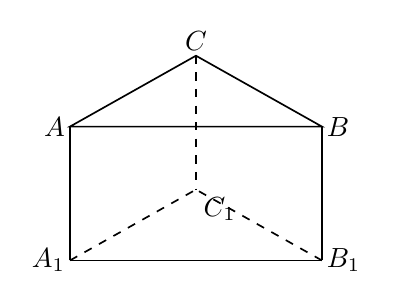
\begin{tikzpicture}[scale=1.0, semithick, every node/.style={inner sep=1.5pt}]
  \coordinate (A) at (-1.60,1.05);
  \coordinate (B) at (1.60,1.05);
  \coordinate (C) at (0.00,1.95);
  \coordinate (A1) at (-1.60,-0.65);
  \coordinate (B1) at (1.60,-0.65);
  \coordinate (C1) at (0.00,0.25);

  \draw (A) -- (B) -- (C) -- cycle;
  \draw (A) -- (A1);
  \draw (B) -- (B1);
  \draw (A1) -- (B1);
  \draw[dashed] (C) -- (C1);
  \draw[dashed] (A1) -- (C1);
  \draw[dashed] (B1) -- (C1);

  \node[left] at (A) {$A$};
  \node[right] at (B) {$B$};
  \node[above] at (C) {$C$};
  \node[left] at (A1) {$A_1$};
  \node[right] at (B1) {$B_1$};
  \node[below right=1pt] at (C1) {$C_1$};
\end{tikzpicture}
